% Sección del Estudiante 2: residuo, error y parada
% Compilar con pdflatex (p. ej. en Overleaf). Las figuras están en ../figuras/
\documentclass[11pt]{article}
\usepackage[spanish,es-noshorthands]{babel}
\usepackage[utf8]{inputenc}
\usepackage[T1]{fontenc}
\usepackage{lmodern}\usepackage{microtype}
\usepackage{amsmath,amssymb,amsthm}
\usepackage{graphicx,booktabs,float}
\usepackage[margin=2.5cm]{geometry}
\usepackage{hyperref}
\graphicspath{{../figuras/}}
\newtheorem{prop}{Proposición}

\title{Residuo, error y criterios de parada en aritmética de punto flotante\\
\large Bisección y punto fijo en Float16, Float32 y Float64}
\author{Estudiante 2 \quad \textit{[nombre del estudiante]}}
\date{Octubre de 2026}

\begin{document}
\maketitle

\section{Pregunta}
Estudiamos tres preguntas relacionadas:
\begin{enumerate}
\item ¿Por qué un residuo pequeño $|f(x_n)|$ no implica que $x_n$ esté cerca de una raíz $r$?
\item ¿Qué sucede en bisección cuando el punto medio ya no se distingue de un extremo en la precisión usada?
\item ¿Qué garantías dan los criterios de parada de bisección y de la iteración de punto fijo $x=F(x)$, y cómo cambian en precisión finita?
\end{enumerate}
Distinguimos siempre el \emph{error hacia adelante} $|x_n-r|$ del \emph{residuo} $|f(x_n)|$.

\section{Marco teórico}

\subsection{Punto flotante}
Un formato binario con $p$ bits de mantisa tiene épsilon de máquina $\varepsilon=2^{1-p}$ y redondeo unitario $u=2^{-p}$; con redondeo al más cercano, $\mathrm{fl}(a\circ b)=(a\circ b)(1+\delta)$, $|\delta|\le u$ \cite{cheney,higham}. Entre $2^e$ y $2^{e+1}$ los flotantes están igualmente espaciados con separación $\mathrm{ulp}=2^{e+1-p}$; en particular, en $[1,2)$ la separación es $\varepsilon$.

\begin{table}[H]\centering
\begin{tabular}{lrrrrr}\toprule
tipo & $p$ & $\varepsilon$ & menor normal & menor subnormal & máximo\\\midrule
Float16 & 11 & $9.77\times10^{-4}$ & $6.10\times10^{-5}$ & $5.96\times10^{-8}$ & $65504$\\
Float32 & 24 & $1.19\times10^{-7}$ & $1.18\times10^{-38}$ & $1.40\times10^{-45}$ & $3.40\times10^{38}$\\
Float64 & 53 & $2.22\times10^{-16}$ & $2.23\times10^{-308}$ & $4.94\times10^{-324}$ & $1.80\times10^{308}$\\\bottomrule
\end{tabular}
\caption{Parámetros IEEE 754 obtenidos con \texttt{eps}, \texttt{floatmin}, \texttt{nextfloat(0)} y \texttt{floatmax} en Julia (tabla 2.0 de \texttt{resultados/exp2\_biseccion\_ulp.md}).}
\end{table}

\subsection{Relación entre residuo y error}
\begin{prop}
Si $r$ es una raíz simple de $f\in C^2$, entonces para $x$ cerca de $r$
\[
|x-r| \;=\; \frac{|f(x)|}{|f'(r)|}\,\bigl(1+O(|x-r|)\bigr).
\]
\end{prop}
\begin{proof}
Por Taylor, $f(x)=f(r)+f'(r)(x-r)+\tfrac12 f''(\xi)(x-r)^2=f'(r)(x-r)\bigl(1+\tfrac{f''(\xi)}{2f'(r)}(x-r)\bigr)$, porque $f(r)=0$. Se despeja $|x-r|$.
\end{proof}
El factor $\kappa=1/|f'(r)|$ es el número de condición absoluto de la raíz: convierte residuo en error. Si $f'(r)$ es pequeño, un residuo diminuto es compatible con un error grande; si $|f'(r)|$ es grande ocurre lo contrario. Para una raíz de multiplicidad $k$, $f(x)\approx \frac{f^{(k)}(r)}{k!}(x-r)^k$, luego
\[
|x-r|\approx\Bigl(\frac{k!\,|f(x)|}{|f^{(k)}(r)|}\Bigr)^{1/k}.
\]
Para $f(x)=(x-1)^7$: $|f(x)|\le 10^{-12}$ se cumple siempre que $|x-1|\le 10^{-12/7}\approx 0.019$.

Además, el criterio $|f(x)|\le\varepsilon_f$ depende de la escala de $f$: $s\,f$ tiene las mismas raíces, pero su residuo es $s$ veces el de $f$. Por último, el $f$ \emph{calculado} no es $f$: cerca de la raíz, $\mathrm{fl}(f(x))=f(x)+\eta(x)$, donde $\eta$ es el error de redondeo de la evaluación. Cuando $|f(x)|<|\eta(x)|$, el signo de $\mathrm{fl}(f(x))$ es ruido \cite{higham}.

\subsection{Bisección}
Si $f(a)f(b)<0$, después de $n$ pasos el punto medio cumple $|m_n-r|\le (b_0-a_0)/2^{n}$ \cite{cheney}: bisección da un \emph{certificado} del error, independiente de $f'$. En aritmética finita:
\begin{itemize}
\item si $a<b$ son flotantes \emph{consecutivos}, no existe ningún flotante entre ellos, así que $\mathrm{fl}((a+b)/2)\in\{a,b\}$ (con redondeo al par más cercano). Desde ese momento el intervalo ya no se reduce;
\item partiendo de $[1,2]$, el ancho tras $k$ pasos es $2^{-k}$, y llega a $1$ ulp $=2^{1-p}$ en $k=p-1$. \textbf{Predicción:} en la iteración $k=p$ (11, 24 y 53) el punto medio coincide con un extremo;
\item si se pide $|b-a|\le\delta$ con $\delta<\mathrm{ulp}(r)$, el criterio nunca se cumple: el ciclo es infinito si no hay un tope de iteraciones. Un criterio alcanzable es relativo, $|b-a|\le 2\varepsilon|m|$, o bien detectar $m=a$ o $m=b$;
\item $(a+b)/2$ se desborda si $a+b>\max$; $a+(b-a)/2$ no;
\item la prueba $f(a)f(m)<0$ falla si el producto da $0$ por underflow; comparar signos con \texttt{sign} evita el problema.
\end{itemize}

\subsection{Punto fijo}
Si $F$ es una contracción en un intervalo $I$ que contiene a $r$ y a los iterados, con $|F'(x)|\le L<1$ en $I$, entonces
\[
|x_n-r|\le \frac{L}{1-L}\,|x_n-x_{n-1}|.
\]
\begin{proof}
$|x_{n-1}-r|\le|x_{n-1}-x_n|+|x_n-r|\le|x_n-x_{n-1}|+L|x_{n-1}-r|$, luego $|x_{n-1}-r|\le|x_n-x_{n-1}|/(1-L)$, y $|x_n-r|=|F(x_{n-1})-F(r)|\le L|x_{n-1}-r|$ por el teorema del valor medio.
\end{proof}
Si $L\approx1$, el factor $L/(1-L)$ es grande: \emph{un paso pequeño no implica un error pequeño}. En los experimentos usamos $L\approx|F'(r)|$, que es una aproximación válida cerca de $r$.

En precisión finita los iterados son $x_{n+1}=\mathrm{fl}(F(x_n))$. Como el conjunto de flotantes es finito, la sucesión calculada termina siendo periódica: puede llegar a un \emph{punto fijo flotante} ($\mathrm{fl}(F(x))=x$) o a un ciclo. Para $F(x)=x-\lambda g(x)$, $\mathrm{fl}(F(x))=x$ ocurre en cuanto $|\lambda g(x)|<\mathrm{ulp}(x)/2$, aunque $x$ esté lejos de $r$. Con $g(x)=x^2-2\approx 2\sqrt2\,(x-\sqrt2)$, la \textbf{predicción} es que la iteración se detiene con
\[
|x-\sqrt2|\approx\frac{\mathrm{ulp}(\sqrt2)}{4\lambda\sqrt2}.
\]

\section{Metodología}
\begin{itemize}
\item \textbf{Lenguaje:} Julia 1.12.6. Bisección, punto fijo y Newton están implementados a mano en \texttt{src/metodos.jl}, de forma genérica en el tipo $T$. Todas las operaciones (punto medio, restas, comparaciones) se hacen en $T$, y las constantes se convierten con \texttt{T(...)} para evitar promociones a Float64.
\item \textbf{Float16:} Julia evalúa cada operación en Float32 y redondea a Float16. Para $+,-,\times,\div,\sqrt{}$ el resultado es idéntico al redondeo directo, porque $24\ge 2\cdot11+2$ \cite{figueroa}. Las funciones $\cos$, $\exp$ y $\arctan$ se evalúan en Float32 y se redondean, así que pueden diferir en 1 ulp de la función correctamente redondeada.
\item \textbf{Referencias:} $r=1$ y $r=0$ son exactas; $\sqrt2$ y la raíz de $x=\cos x$ se calcularon en BigFloat de 256 bits (la segunda con Newton, iterando hasta un paso $<2^{-246}$). El error $|x-r|$ se evaluó convirtiendo $x$ exactamente a BigFloat. Así, el error de la referencia ($\lesssim10^{-70}$) es despreciable frente a cualquier error reportado.
\item \textbf{Registro:} en cada iteración se guardan $x_n$ (o $a,b,m$), el residuo, el paso o el ancho y el error. Cada ejecución reporta el \emph{estado} final: \texttt{tol\_x}, \texttt{tol\_f}, \texttt{residuo\_cero} ($\mathrm{fl}(f(m))=0$), \texttt{estancado} ($m=a$ o $m=b$), \texttt{punto\_fijo\_flotante}, \texttt{ciclo}, \texttt{no\_finito} o \texttt{max\_iter}.
\item \sloppy\textbf{Reproducibilidad:} \texttt{exp1\_residuo\_error.jl}, \texttt{exp2\_biseccion\_ulp.jl}, \texttt{exp3\_punto\_fijo.jl} y \texttt{graficos.jl}; las tablas completas están en \texttt{resultados/}.
\end{itemize}

\section{Resultados}

\subsection{Experimento 1: residuo pequeño no implica error pequeño}
\textbf{Funciones.} $\arctan(x-1)$ (raíz simple con $f'(1)=1$, bien condicionada); $(x-1)^7$ en forma factorizada y desarrollada (evaluada con Horner); $x e^{-x}$ (raíz $0$, pero $f\to0$ cuando $x\to\infty$); y $s(x^2-2)$ para estudiar la escala.

\begin{figure}[H]\centering
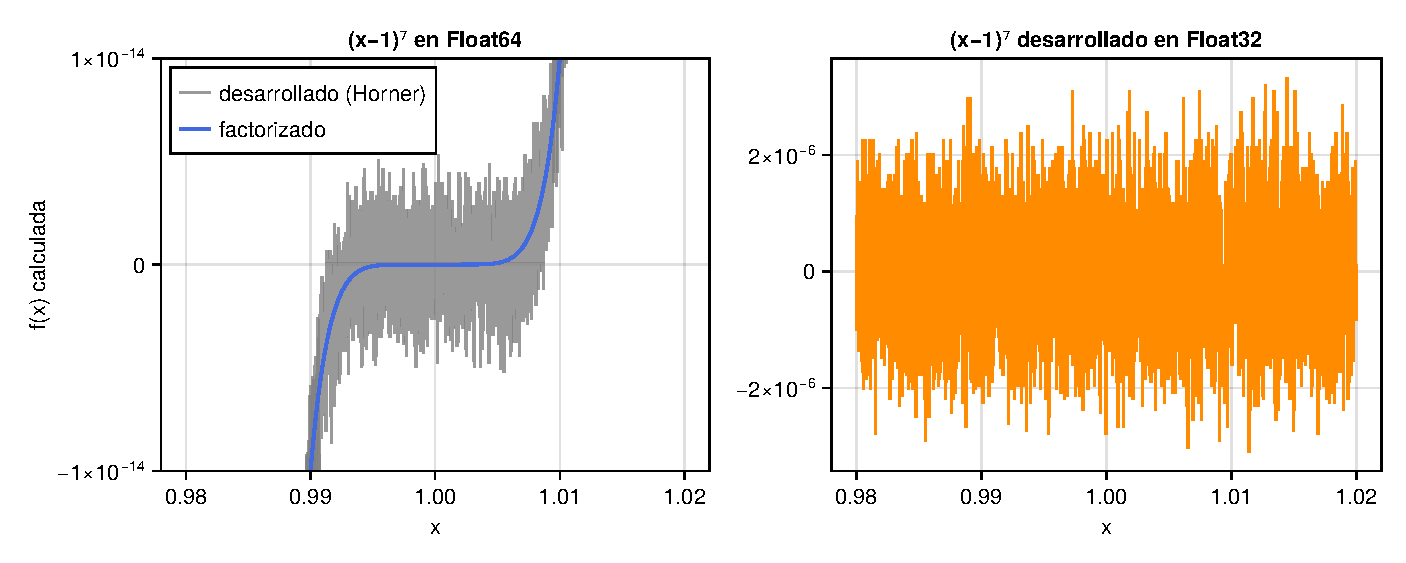
\includegraphics[width=\textwidth]{fig1_ruido_f7.pdf}
\caption{$(x-1)^7$ calculado en $[0.98,1.02]$. La forma desarrollada produce ruido de redondeo de amplitud $\sim10^{-15}$ (Float64) y $\sim10^{-6}$ (Float32). En 4001 puntos, la función real cambia de signo 1 vez; la forma desarrollada cambia 717 veces en Float64 y 1955 en Float32.}
\end{figure}

\begin{table}[H]\centering\footnotesize\setlength{\tabcolsep}{4pt}
\begin{tabular}{llllrlll}\toprule
tipo & $f$ & $\varepsilon_f$ & estado & iter & $x$ final & $|f(x)|$ & $|x-1|$\\\midrule
Float16 & $(x-1)^7$ fact. & $6\times10^{-8}$ & residuo\_cero & 3 & 0.9497 & 0 & $5.0\times10^{-2}$\\
Float16 & $(x-1)^7$ desarr. & $6\times10^{-8}$ & estancado & 12 & 0.6543 & $3.4\times10^{-3}$ & $3.5\times10^{-1}$\\
Float32 & $(x-1)^7$ fact. & $10^{-12}$ & tol\_f & 5 & 0.9875001 & $4.8\times10^{-14}$ & $1.3\times10^{-2}$\\
Float32 & $(x-1)^7$ desarr. & $10^{-12}$ & estancado & 26 & 0.9161725 & $6.0\times10^{-8}$ & $8.4\times10^{-2}$\\
Float64 & $\arctan(x-1)$ & $10^{-12}$ & tol\_f & 39 & 0.99999999999927 & $7.3\times10^{-13}$ & $7.3\times10^{-13}$\\
Float64 & $(x-1)^7$ fact. & $10^{-12}$ & tol\_f & 5 & 0.9875 & $4.8\times10^{-14}$ & $1.3\times10^{-2}$\\\bottomrule
\end{tabular}
\caption{Bisección en $[0.5,1.7]$ deteniéndose por residuo (extracto de la tabla 1B).}
\end{table}

\textbf{Observaciones.}
(i) Para $\arctan$ el error coincide con el residuo, como predice $\kappa=1$.
(ii) Para $(x-1)^7$, un residuo $<10^{-12}$ se alcanza con solo 2 dígitos correctos, en la iteración 5, tal como predice $0.019$.
(iii) En Float16 el residuo es \emph{exactamente} $0$ en $x=0.9497$: $(-0.0503)^7\approx-8\times10^{-10}$ es menor que el menor subnormal ($6\times10^{-8}$), así que hubo underflow. Un residuo cero no certifica una raíz.
(iv) Con la forma desarrollada en Float32, bisección sigue signos que son ruido y termina en $0.916$, con error $0.08$.

\begin{figure}[H]\centering
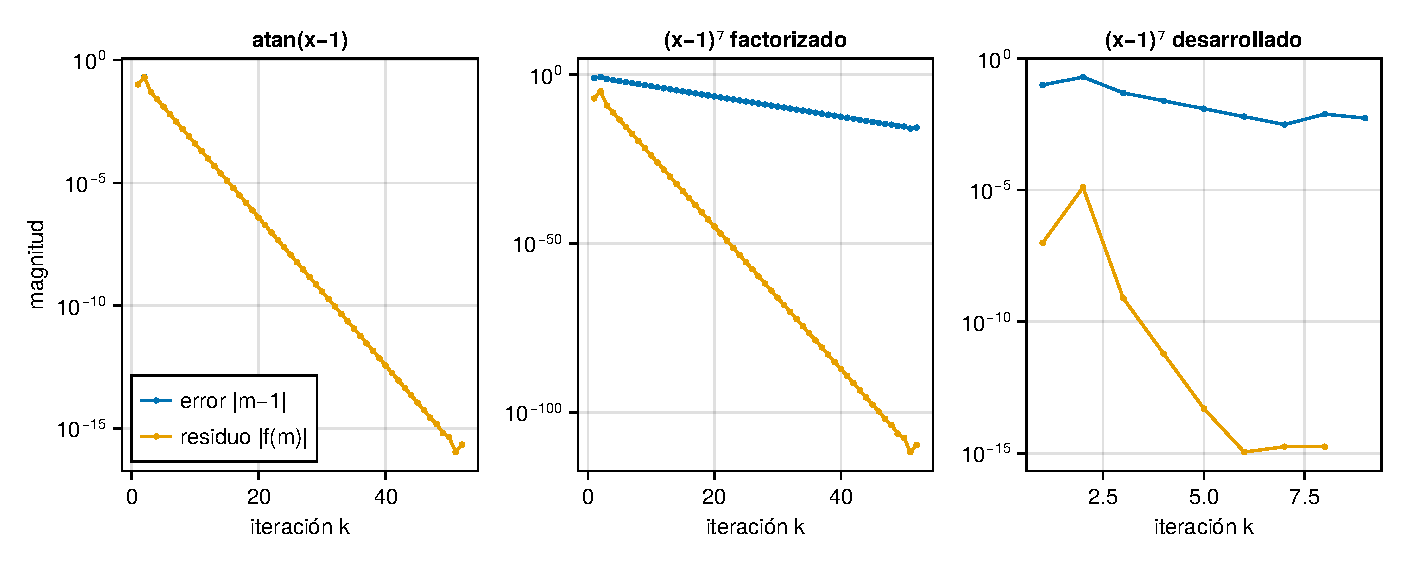
\includegraphics[width=\textwidth]{fig2_residuo_vs_error.pdf}
\caption{Error y residuo por iteración de bisección (Float64, solo con parada por residuo exactamente cero o estancamiento). En la forma factorizada el residuo baja hasta $10^{-100}$ mientras el error baja a la séptima parte de esa velocidad en escala log; en la forma desarrollada $\mathrm{fl}(f(m))=0$ exactamente en $m=0.99453$ (iteración 9), con error $5.5\times10^{-3}$.}
\end{figure}

\textbf{Newton en $xe^{-x}$ desde $x_0=2$, con parada $|f(x_n)|\le10^{-6}$.} En las tres precisiones la iteración se aleja de la raíz: el método se detiene en $x\approx17.6$ (Float32 y Float64, 13 iteraciones) o en $x=16.53$ (Float16, 12 iteraciones), con residuo $<10^{-6}$ y error $\approx17$ (figura~\ref{fig:xexp}). Esto es una \emph{falsa convergencia}: el criterio de residuo se cumple porque $f\to0$ en el infinito, no porque haya una raíz.

\begin{figure}[H]\centering
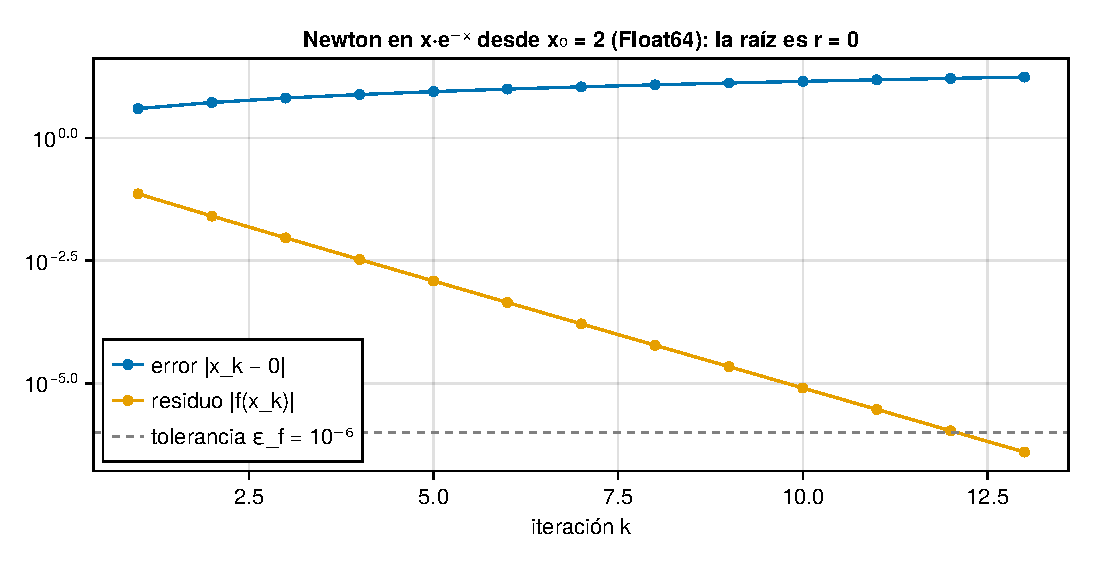
\includegraphics[width=.7\textwidth]{fig6_newton_xexp.pdf}
\caption{Newton en $xe^{-x}$: el residuo cae mientras el error crece.}\label{fig:xexp}
\end{figure}

\begin{table}[H]\centering
\begin{tabular}{rrlrll}\toprule
$s$ & $\kappa=1/|f'(r)|$ & estado & iter & $|f(x)|$ & $|x-\sqrt2|$\\\midrule
$10^{-10}$ & $3.5\times10^{9}$ & tol\_f & 1 & $2.5\times10^{-11}$ & $8.6\times10^{-2}$\\
$10^{-4}$ & $3.5\times10^{3}$ & tol\_f & 13 & $8.2\times10^{-9}$ & $2.9\times10^{-5}$\\
$1$ & $0.35$ & tol\_f & 27 & $5.2\times10^{-9}$ & $1.9\times10^{-9}$\\
$10^{8}$ & $3.5\times10^{-9}$ & estancado & 53 & $4.4\times10^{-8}$ & $1.3\times10^{-16}$\\\bottomrule
\end{tabular}
\caption{Misma raíz, distinta escala: bisección de $s(x^2-2)$ en Float64 con $\varepsilon_f=10^{-8}$. En todos los casos, error $\approx\kappa\cdot$residuo.}
\end{table}
Con $s=10^{8}$ la tolerancia de residuo es \emph{inalcanzable}: el error ya es menor que 1 ulp, y aun así el residuo es $4.4\times10^{-8}>10^{-8}$. Sin la detección de estancamiento el ciclo no terminaría.

\subsection{Experimento 2: el punto medio que no se distingue de un extremo}
\begin{table}[H]\centering\footnotesize\setlength{\tabcolsep}{4pt}
\begin{tabular}{lrlrlllc}\toprule
tipo & $p$ & estado & iter & $a$ final & $b$ final & $b-a$ & ¿consecutivos?\\\midrule
Float16 & 11 & estancado & 11 & 1.413 & 1.414 & $9.77\times10^{-4}$ & sí\\
Float32 & 24 & estancado & 24 & 1.4142135 & 1.4142137 & $1.19\times10^{-7}$ & sí\\
Float64 & 53 & estancado & 53 & 1.414213562373095 & 1.4142135623730951 & $2.22\times10^{-16}$ & sí\\\bottomrule
\end{tabular}
\caption{Bisección de $x^2-2$ en $[1,2]$ con $\delta=0$. El estancamiento ocurre exactamente en la iteración $p$, como se predijo.}
\end{table}

\begin{figure}[H]\centering
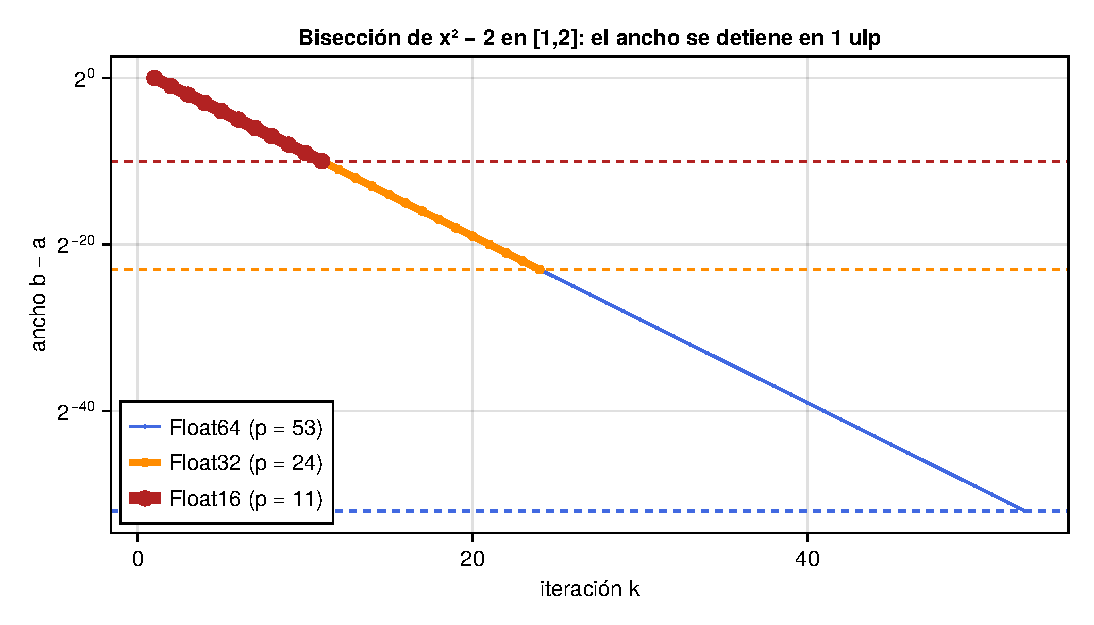
\includegraphics[width=.7\textwidth]{fig3_biseccion_ulp.pdf}
\caption{Ancho $b-a$ por iteración; las líneas discontinuas marcan $2^{1-p}$.}
\end{figure}

\textbf{Tolerancias inalcanzables (tabla 2B).} Con $\delta=10^{-10}$ absoluto y sin detectar el estancamiento:
en Float32 el método llega al tope de 200 iteraciones, porque $\mathrm{ulp}(\sqrt2)=1.2\times10^{-7}>\delta$; en Float64 termina en 34 iteraciones.
Para $x^2-2\cdot10^{12}$ en $[10^6,2\cdot10^6]$, incluso Float64 llega al tope de 200: $\mathrm{ulp}(1.4\times10^6)=2.3\times10^{-10}>10^{-10}$. Una tolerancia absoluta no tiene sentido sin mirar la magnitud de la raíz. El criterio relativo $|b-a|\le2\varepsilon|m|$ termina en 23 (Float32) y 52 (Float64) iteraciones.

\textbf{Residuo cero en Float16.} En Float16, $\mathrm{fl}(1.414^2)=2$, así que $\mathrm{fl}(f(1.414))=0$ con error $1.5\times10^{-4}$. Si no se desactiva la parada por residuo cero, la bisección se detiene allí en la iteración 7 (tabla 2E).

\textbf{Desbordamiento y underflow (tablas 2C y 2D).}
En Float16 con $[60000,65000]$, $(a+b)/2$ da \texttt{Inf} en la primera iteración y $a+(b-a)/2$ funciona; en Float64 con $[10^{308},1.7\cdot10^{308}]$ pasa lo mismo.
Con $f=10^{-3}(x^2-2)$ en Float16, la prueba $f(a)f(m)<0$ descarta el subintervalo correcto en cuanto el producto se anula por underflow, y termina en $x=1.5$ (error $0.086$); con \texttt{sign} se obtiene $1.414$.
Lo mismo ocurre en Float64 con $10^{-160}(x^2-2)$: el error es $7.7\times10^{-3}$ frente a $1.3\times10^{-16}$.

\subsection{Experimento 3: punto fijo frente a bisección}
\textbf{$x=\cos x$}, $x_0=1$, con $L=\sin r\approx0.674$ y $L/(1-L)\approx2.06$.
En todas las ejecuciones con $\delta\in\{10^{-3},10^{-6},10^{-10}\}$, el error real quedó por debajo de la cota $\frac{L}{1-L}|x_n-x_{n-1}|$ (tabla 3A).
Para la misma tolerancia, bisección en $[0,1]$ necesita casi la mitad de iteraciones (9, 19 y 33 frente a 17, 34 y 58 en Float64), y su cota no depende de estimar $L$.
Si se itera con $\delta=0$, aparecen los efectos de la precisión finita:
\begin{itemize}
\item Float16: \textbf{ciclo de periodo 2}, $0.7393\leftrightarrow0.739$, con error $3.2\times10^{-4}$. El paso nunca baja de 1 ulp, así que $|x_n-x_{n-1}|\le10^{-6}$ nunca se cumpliría;
\item Float32: también un ciclo de periodo 2, $0.7390851\leftrightarrow0.7390852$;
\item Float64: punto fijo flotante exacto tras 91 iteraciones, con error $3\times10^{-17}$, menor que 1 ulp.
\end{itemize}

\begin{figure}[H]\centering
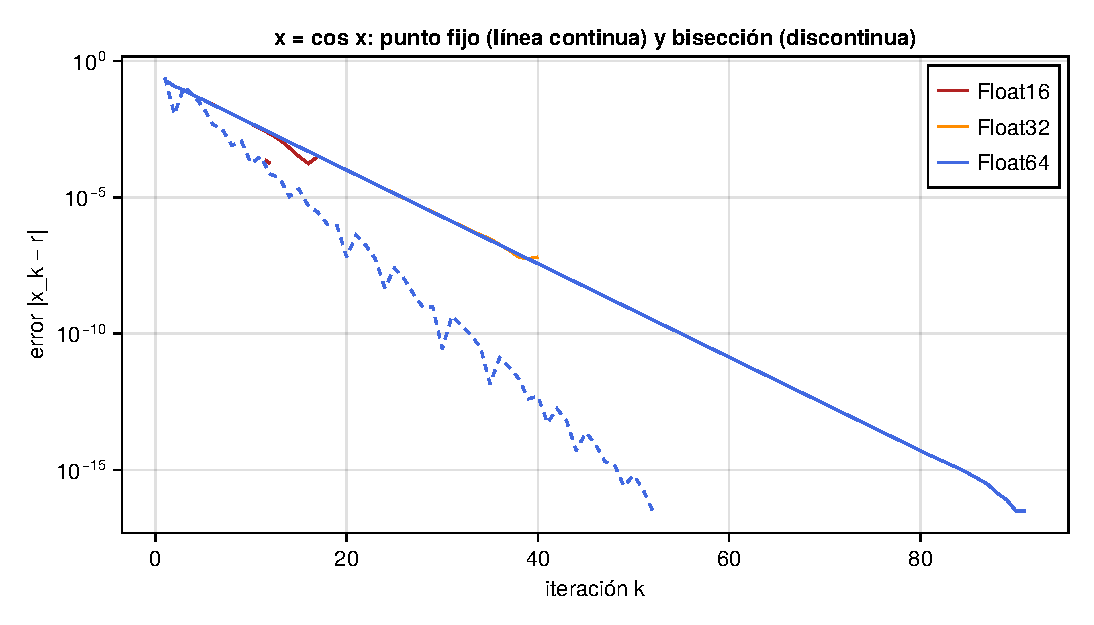
\includegraphics[width=.7\textwidth]{fig4_cos_pf_vs_biseccion.pdf}
\caption{$x=\cos x$: error de punto fijo y de bisección en las tres precisiones.}
\end{figure}

\textbf{Contracción lenta} $F(x)=x-10^{-3}(x^2-2)$, con $L=F'(\sqrt2)\approx0.99717$ y $L/(1-L)\approx353$.
\begin{table}[H]\centering\small
\begin{tabular}{llrrlll}\toprule
tipo & $\delta$ & estado & iter & último paso & $|x-\sqrt2|$ & cota\\\midrule
Float64 & $10^{-6}$ & tol\_x & 2552 & $1.0\times10^{-6}$ & $3.5\times10^{-4}$ & $3.5\times10^{-4}$\\
Float64 & $10^{-8}$ & tol\_x & 4178 & $1.0\times10^{-8}$ & $3.5\times10^{-6}$ & $3.5\times10^{-6}$\\
Float32 & $10^{-8}$ & punto fijo flot. & 3507 & 0 & $2.1\times10^{-5}$ & ---\\
Float16 & cualquiera & punto fijo flot. & 237 & 0 & $1.8\times10^{-1}$ & ---\\\bottomrule
\end{tabular}
\caption{Extracto de la tabla 3B. El criterio de paso se cumple con un error real $\approx350$ veces mayor que la tolerancia.}
\end{table}

\begin{table}[H]\centering
\begin{tabular}{lrll}\toprule
tipo & iter & $|x-\sqrt2|$ observado & predicción $\mathrm{ulp}(\sqrt2)/(4\lambda\sqrt2)$\\\midrule
Float16 & 237 & $1.84\times10^{-1}$ & $1.73\times10^{-1}$\\
Float32 & 3507 & $2.101\times10^{-5}$ & $2.107\times10^{-5}$\\
Float64 & 10604 & $3.921\times10^{-14}$ & $3.925\times10^{-14}$\\\bottomrule
\end{tabular}
\caption{Error al que la iteración se detiene porque $\mathrm{fl}(F(x))=x$. La predicción coincide con lo observado (en Float16 la aproximación lineal $x^2-2\approx2\sqrt2(x-\sqrt2)$ es menos precisa, porque $x$ está lejos de $\sqrt2$).}
\end{table}
En Float32 la iteración se \emph{detiene exactamente} ($x_{n+1}=x_n$, paso $0$) con 4 dígitos correctos. Desde el punto de vista del criterio, eso es una "convergencia perfecta" que no lo es.

\begin{figure}[H]\centering
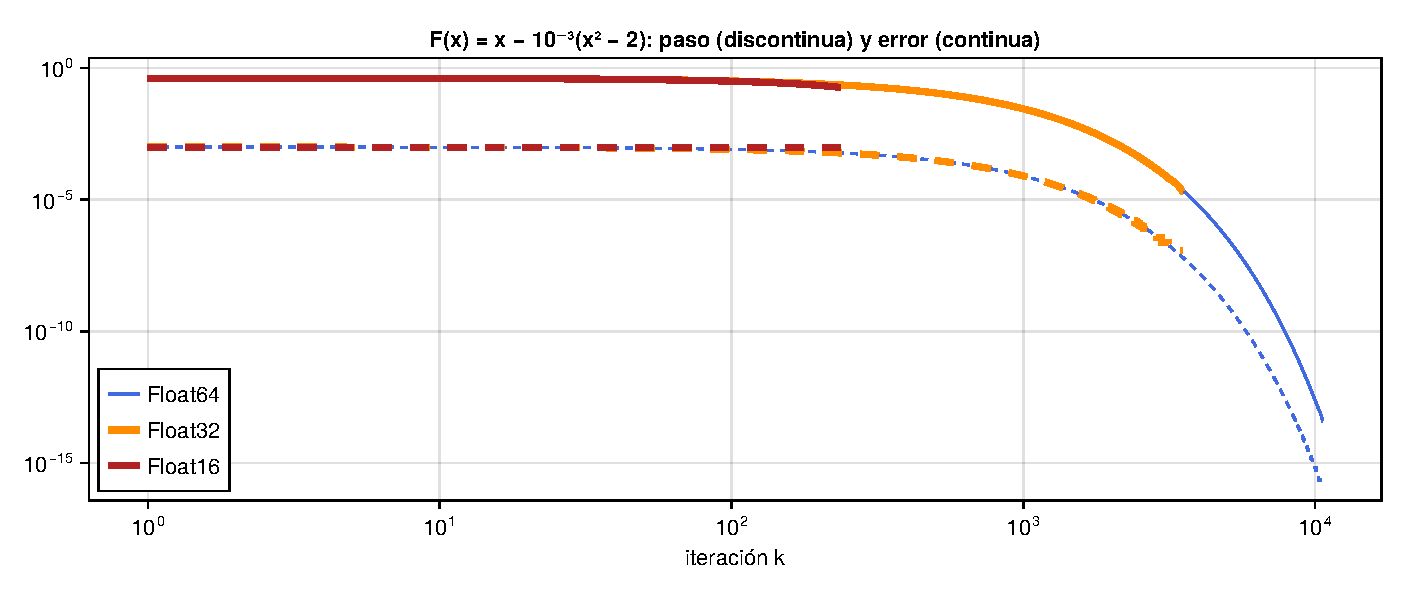
\includegraphics[width=\textwidth]{fig5_contraccion_lenta.pdf}
\caption{Paso (discontinua) y error (continua). La distancia vertical constante entre ambas curvas (en escala log) es el factor $\approx L/(1-L)\approx 353$; las curvas terminan cuando se alcanza el punto fijo flotante.}
\end{figure}

\section{Discusión}
\begin{itemize}
\item \textbf{Residuo y error miden cosas distintas.} El residuo mide qué tan bien $x$ satisface la ecuación, y el error qué tan cerca está de la solución; los relaciona $\kappa=1/|f'(r)|$, que es una propiedad del problema y no del método. Las raíces múltiples ($(x-1)^7$), las funciones con asíntota en cero ($xe^{-x}$) y el escalamiento ($s\,f$) muestran que $|f(x)|\le\varepsilon_f$ por sí solo no garantiza nada sobre $|x-r|$.
\item \textbf{El $f$ calculado no es $f$.} Underflow (Float16), cancelación en la forma desarrollada y redondeo ($\mathrm{fl}(1.414^2)=2$) pueden producir residuos exactamente nulos o signos aleatorios. Bisección converge a un cambio de signo del $f$ \emph{calculado}, que puede estar lejos de la raíz real.
\item \textbf{Bisección: la precisión fija el límite.} El ancho no puede bajar de 1 ulp de la raíz, y lo alcanza en exactamente $p$ pasos desde $[1,2]$. Toda tolerancia absoluta menor que $\mathrm{ulp}(r)$ produce un ciclo infinito; por eso hay que usar una tolerancia relativa, detectar $m\in\{a,b\}$ y fijar un número máximo de iteraciones.
\item \textbf{Punto fijo: el paso solo informa si se conoce $L$.} Con $L\approx1$ el paso subestima el error en un factor $1/(1-L)$. En precisión finita, además, la sucesión puede detenerse en un punto fijo flotante lejos de $r$, o ciclar, de modo que un criterio de paso puede declarar convergencia (paso $0$) o no cumplirse nunca (ciclo).
\item \textbf{Respuesta a la pregunta de ensayo} (¿por qué Float32 se estanca cerca de $10^{-7}$?): en $[1,2)$ los flotantes de precisión simple están separados por $2^{-23}\approx1.2\times10^{-7}$. Bisección se detiene allí (iteración 24, $a$ y $b$ consecutivos) porque no hay más números entre ellos; en Float64 la separación es $2.2\times10^{-16}$ y el método puede avanzar hasta la iteración 53.
\end{itemize}

\section{Conclusiones y aprendizajes}
\begin{enumerate}
\item \textbf{El residuo no es una medida del error.} Están relacionados por $|x-r|\approx|f(x)|/|f'(r)|$, así que la información que da el residuo depende del condicionamiento de la raíz. Con $(x-1)^7$ un residuo de $5\times10^{-14}$ correspondió a solo 2 dígitos correctos; con $xe^{-x}$, Newton cumplió $|f|\le10^{-6}$ a distancia 17 de la única raíz; y con $s(x^2-2)$ el mismo criterio absoluto se cumplió en 1 iteración ($s=10^{-10}$) o nunca ($s=10^{8}$). Un criterio de residuo solo tiene sentido si se interpreta junto con $|f'|$ y con la escala de $f$.
\item \textbf{Se resuelve la ecuación calculada, no la real.} Cerca de la raíz, $\mathrm{fl}(f(x))$ puede ser ruido (717 cambios de signo de $(x-1)^7$ desarrollado en Float64) o exactamente cero por underflow o redondeo (Float16). Bisección encuentra un cambio de signo de $\mathrm{fl}(f)$, que puede estar lejos de $r$. Por eso conviene evaluar $f$ en una forma estable (factorizada) cuando se pueda.
\item \textbf{La precisión fija un piso y el algoritmo debe reconocerlo.} En bisección el intervalo no puede ser menor que un ulp, y desde $[1,2]$ eso ocurre exactamente en la iteración $p$ (11, 24 y 53). En punto fijo, la iteración termina en un punto fijo flotante o en un ciclo de periodo 2. Las tolerancias absolutas menores que $\mathrm{ulp}(r)$ producen ciclos infinitos: lo vimos en Float32 y, para una raíz de magnitud $10^6$, incluso en Float64.
\item \textbf{Un paso pequeño no es un error pequeño.} En punto fijo el error es del orden de $\frac{L}{1-L}$ veces el paso. Con $L=0.997$, parar con $|x_n-x_{n-1}|\le10^{-8}$ dejó un error de $3.5\times10^{-6}$. Bisección, en cambio, entrega una cota del error que no depende de $f'$ ni de $L$, y en $x=\cos x$ usó menos iteraciones que punto fijo para la misma tolerancia.
\item \textbf{Detalles de implementación que cambian el resultado:} $a+(b-a)/2$ en lugar de $(a+b)/2$ (evita \texttt{Inf}), comparar signos con \texttt{sign} en lugar de $f(a)f(m)<0$ (evita el underflow) y registrar el criterio de parada que se activó en cada ejecución.
\end{enumerate}
\textbf{Recomendación práctica.} Un criterio de parada robusto combina: tolerancia relativa en $x$ (no menor que unos pocos $\varepsilon|x|$), residuo interpretado con $|f'|$, detección de estancamiento ($m\in\{a,b\}$, $x_{n+1}=x_n$ o ciclo), control de \texttt{NaN}/\texttt{Inf} y un número máximo de iteraciones. Además, siempre hay que reportar cuál de ellos detuvo el método.

\textbf{Aprendizaje sobre el método de trabajo.} Escribir la predicción antes de correr el experimento (iteración $p$, error $\mathrm{ulp}(\sqrt2)/(4\lambda\sqrt2)$) permitió distinguir lo que la teoría explica de lo que fue sorpresa: el underflow que da residuo cero en Float16 y los ciclos de periodo 2 no estaban previstos y obligaron a ajustar la explicación.

\section{Declaración de uso de IA}
\textbf{Herramienta:} Claude (modelo Opus 5.5, Anthropic), usado mediante Claude Code (aplicación de escritorio) el 16 de octubre de 2026, con acceso al repositorio del curso y a una instalación local de Julia.

\textbf{Qué hizo la IA.} Leyó la guía de trabajo, propuso los casos de prueba y las predicciones teóricas, escribió el código Julia (\texttt{src/metodos.jl}, los tres scripts de experimentos y \texttt{graficos.jl}), lo ejecutó, generó las figuras y redactó este informe, incluidas las conclusiones. \emph{Las conclusiones y los aprendizajes fueron redactados por la IA a partir de los resultados obtenidos, por petición expresa del estudiante, y el estudiante los revisó y asume la responsabilidad de defenderlos.}

\textbf{Prompts relevantes} (mensajes del estudiante, en orden):
\begin{enumerate}
\item ``Hola tengo que hacer esta investigación [\dots] para lo cual tengo este repo: \url{https://github.com/archeyne/NonlinearEquations-FloatingPoint-AN2026} [\dots] soy el estudiante 2. Hagamos juntos la investigación y hazme preguntas y charlamos y hacemos lo que tenemos que hacer.'' (Se adjuntó el enunciado de la tarea.)
\item Respuestas a las preguntas de la IA: lenguaje \emph{Julia}; bibliografía \emph{Cheney \& Kincaid}; entrega en \emph{PDF y scripts de experimentación, al GitHub}; plazo \emph{día 3, urgente}.
\item ``Instala TinyTeX en este computador y compila el PDF aquí.''
\item ``Completemos las cosas que hacen falta, los prompts sin completar para que se haga una buena integración.'' Y luego: ``pon tus conclusiones no tengo tiempo''.
\item ``Haz commit de la carpeta estudiante2 y súbela al repositorio de GitHub.''
\end{enumerate}

\textbf{Verificaciones y correcciones realizadas.}
\begin{itemize}
\item Todos los números del informe se obtuvieron ejecutando los scripts; ninguno fue escrito a mano por la IA. Las tablas completas están en \texttt{resultados/*.md}.
\item Cada afirmación teórica se contrastó con una predicción cuantitativa: estancamiento en la iteración $p$ (observado: 11, 24 y 53); error de estancamiento $\mathrm{ulp}(\sqrt2)/(4\lambda\sqrt2)$ (Float32: $2.107\times10^{-5}$ predicho frente a $2.101\times10^{-5}$ observado); cota $L/(1-L)$ (se cumplió en todas las ejecuciones de la tabla 3A).
\item Errores encontrados y corregidos durante el trabajo: (i) la primera versión de bisección se detenía cuando $|f(m)|\le0$ con la tolerancia por defecto, lo que ocultaba el estancamiento en Float16; se separó la parada por residuo cero (\texttt{parar\_cero}). (ii) El conteo de cambios de signo ignoraba el cruce exacto por $0$ (daba 0 para la forma factorizada); se corrigió para dar 1. (iii) En las figuras 1, 3 y 5 las curvas de Float16 y Float32 quedaban ocultas; se cambió el orden y el grosor de las líneas.
\item En el documento previo \texttt{investiacion\_precision.txt} del repositorio (generado con IA) se detectó un error: dice $\varepsilon\approx2^{-11}\approx9.77\times10^{-4}$ para Float16, pero el épsilon de máquina es $2^{-10}\approx9.77\times10^{-4}$, mientras que $2^{-11}\approx4.88\times10^{-4}$ es el redondeo unitario. Se verificó con \texttt{eps(Float16)} en Julia.
\item Los datos bibliográficos de \cite{cheney} y \cite{figueroa} se verificaron en la página de la editorial y en un listado de referencias con DOI. La afirmación sobre el doble redondeo en Float16 se apoya además en \cite{roux}.
\end{itemize}

\begin{thebibliography}{99}
\bibitem{cheney} W. Cheney y D. Kincaid, \emph{Numerical Mathematics and Computing}, 7.ª ed., Brooks/Cole, Cengage Learning, 2013. (Cap. 1: aritmética de punto flotante; cap. 3: localización de raíces.)
\bibitem{higham} N. J. Higham, \emph{Accuracy and Stability of Numerical Algorithms}, 2.ª ed., SIAM, 2002.
\bibitem{goldberg} D. Goldberg, ``What every computer scientist should know about floating-point arithmetic'', \emph{ACM Computing Surveys} 23(1):5--48, 1991.
\bibitem{figueroa} S. A. Figueroa, ``When is double rounding innocuous?'', \emph{ACM SIGNUM Newsletter} 30(3):21--26, 1995. doi:10.1145/221332.221334.
\bibitem{roux} P. Roux, ``Innocuous double rounding of basic arithmetic operations'', \emph{Journal of Formalized Reasoning}, 2014.
\bibitem{ieee} IEEE Std 754-2019, \emph{IEEE Standard for Floating-Point Arithmetic}, 2019.
\bibitem{julia} Documentación de Julia, ``Integers and Floating-Point Numbers'', \url{https://docs.julialang.org/en/v1/manual/integers-and-floating-point-numbers/}.
\end{thebibliography}
\end{document}
